\documentclass[12pt,a4paper]{article}
\usepackage[utf8]{inputenc}
%Set page layout parameters
\usepackage[
top=4cm,
bottom=2cm,
left=2cm,
right=2cm,
headheight=2cm,
footskip=1cm,
marginparwidth=2cm]{geometry}
\usepackage[dvipsnames]{xcolor}
% To use color boxes
\usepackage{tcolorbox}
\usepackage{lipsum}
\tcbuselibrary{listings,theorems,skins,vignette,raster,breakable,magazine,poster,fitting,hooks}
\newcounter{ejemplo}
%Images path
\graphicspath{{images/}}
\usepackage{float} %provide us with the option H
\usepackage{fancyhdr}
\usepackage{tikz}
\usetikzlibrary{automata, positioning, arrows}
\usepackage{tikzpagenodes}
%to redefine figure caption 
\renewcommand{\figurename}{Figura}
%change text font
\usepackage[T1]{fontenc}
\usepackage{tgbonum} % LaTeX will use the TEX Gyre Bonum font family

\definecolor{subtitle_yellow}{RGB}{252,213,129}
\definecolor{title_yellow}{RGB}{249,175,16}
\definecolor{steel_blue_title}{RGB}{93,138,168}
\definecolor{pewter_blue_subtitle}{RGB}{149,178,198}
\definecolor{ecru_circle}{RGB}{215,190,130}
\definecolor{ecru_circle1}{RGB}{68,148,173}

\newcommand{\myfirststyle}{%
	\begin{tikzpicture}[remember picture, overlay]
		
		%top border
		\fill[fill=steel_blue_title](current page.north west) rectangle ([yshift=-15mm]current page.north east);
		
		\fill[fill=pewter_blue_subtitle]([yshift=-17mm]current page.north west) rectangle ([yshift=-30mm]current page.north east);
		
		%page box
		%\draw[lightgray, fill=Rhodamine, fill opacity=0.05, line width=1mm, rounded corners=3mm] ([xshift=-5mm,yshift=5mm]current page text area.north west) rectangle ([xshift=5mm,yshift=-5mm]current page text area.south east);
		
		%bottom box
		\fill[fill=pewter_blue_subtitle](current page.south west) rectangle ([yshift=10mm]current page.south east);
		
		%page circle
		\draw[white,fill=ecru_circle1,line width=2mm] ([xshift=-5mm,yshift=25mm]current page text area.north east) circle (1); 
		
		
		%page number text        
		%\node[anchor=center] at ([xshift=-5mm,yshift=25mm]current page text area.north east) {\Huge\bfseries\sffamily\color{white}{\thepage}};
		
		%title text
		\node[anchor=west] at ([yshift=32mm]current page text area.north west) {\Huge\bfseries\sffamily\color{white}{Resistores en serie}};
		
		%subtitle text
		\node[anchor=west] at ([xshift=10mm,yshift=16mm]current page text area.north west) {\Large\bfseries\sffamily\color{white}{Divisor de tensión}};
		
		%footer text
		\node[anchor=center] at ([yshift=-15mm]current page text area.south) {\large\bfseries\sffamily\color{white}{Created by: Rodrigo Castillejos}};
		
	\end{tikzpicture}
}


%create page style
\fancypagestyle{MyFirstStyle}{%
	\fancyhf{}
	\fancyhead[C]{\myfirststyle}
	\renewcommand{\headrulewidth}{0pt}
}%

\pagestyle{MyFirstStyle}

\colorlet{colexam}{red!75!black}
\newtcolorbox[use counter=ejemplo]{myexample}{%
	empty,title={Ejemplo \thetcbcounter},attach boxed title to top left,
	boxed title style={empty,size=minimal,toprule=2pt,top=4pt,
		overlay={\draw[colexam,line width=2pt]
			([yshift=-1pt]frame.north west)--([yshift=-1pt]frame.north east);}},
	coltitle=colexam,fonttitle=\Large\bfseries,
	before=\par\medskip\noindent,parbox=false,boxsep=0pt,left=0pt,right=3mm,top=4pt,
	breakable,pad at break*=0mm,vfill before first,
	overlay unbroken={\draw[colexam,line width=1pt]
		([yshift=-1pt]title.north east)--([xshift=-0.5pt,yshift=-1pt]title.north-|frame.east)
		--([xshift=-0.5pt]frame.south east)--(frame.south west); },
	overlay first={\draw[colexam,line width=1pt]
		([yshift=-1pt]title.north east)--([xshift=-0.5pt,yshift=-1pt]title.north-|frame.east)
		--([xshift=-0.5pt]frame.south east); },
	overlay middle={\draw[colexam,line width=1pt] ([xshift=-0.5pt]frame.north east)
		--([xshift=-0.5pt]frame.south east); },
	overlay last={\draw[colexam,line width=1pt] ([xshift=-0.5pt]frame.north east)
		--([xshift=-0.5pt]frame.south east)--(frame.south west);},%
}

\tikzset{
	->, %makes the edges directed
	>=stealth, % makes the arrow heads bold
	node distance=3cm, % specifies the mininum distance between two nodes. Change if necessary
	every state/.style={thick, fill=gray!10}, %sets the properties for each 'state' node
	initial text=$ $, %sets the text that appears on the start arrow 
}

\begin{document}
	\begin{figure}[ht]\centering
		\begin{tikzpicture}
			\path (0,2)  node [shape=circle,draw] {}
				  (0,1)  node [shape=circle,draw] {}
				  (0,0)  node [shape=circle,draw] {}
				  (1,1)  node [shape=rectangle,draw] {}
				  (-1,1) node [shape=rectangle,draw] {};
		\end{tikzpicture}
	\caption{Caption of the FSM}
	\end{figure}

	\begin{figure}[ht]\centering
		\begin{tikzpicture}
			\node at (0,2)  [circle,draw] {};
			\node at (0,1)  [circle,draw] {};
			\node at (0,0)  [circle,draw] {};
			\node at (1,1)  [rectangle,draw] {};
			\node at (-1,1) [rectangle,draw] {};
		\end{tikzpicture}
		\caption{Caption of the FSM}
	\end{figure}

	\begin{figure}[ht]\centering
		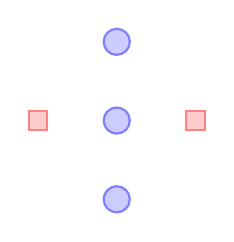
\begin{tikzpicture}[thick]
			\node at (0,2)  [circle,draw=blue!50,fill=blue!20] {};
			\node at (0,1)  [circle,draw=blue!50,fill=blue!20] {};
			\node at (0,0)  [circle,draw=blue!50,fill=blue!20] {};
			\node at (1,1)  [rectangle,draw=red!50,fill=red!20] {};
			\node at (-1,1) [rectangle,draw=red!50,fill=red!20] {};
		\end{tikzpicture}
		\caption{Caption of the FSM}
	\end{figure}

	\begin{figure}[H]\centering
		\tikzstyle{place} = [circle,draw=blue!50,fill=blue!20,thick]
		\tikzstyle{transition} = [rectangle,draw=red!50,fill=red!20,thick]
		\begin{tikzpicture}[thick]
			\node at (0,2)  [place] {};
			\node at (0,1)  [place] {};
			\node at (0,0)  [place] {};
			\node at (1,1)  [transition] {};
			\node at (-1,1) [transition] {};
		\end{tikzpicture}
		\caption{Caption of the FSM}
	\end{figure}

	\begin{figure}[H]\centering
		\tikzstyle{hello} = [circle,draw=blue!50,fill=blue!20,thick,inner sep=0pt,minimum size=6mm]
		\tikzstyle{transition} = [rectangle,draw=red!50,fill=red!20,thick,inner sep=0pt,minimum size=5mm]
		\begin{tikzpicture}[thick]
			\node[hello] (waiting 1) at (0,2) {};
			\node[hello] (critical 1) at (0,1) {};
			\node[hello] (semaphore) at (0,0) {};
			\node[transition] (leaving critical) at (1,1) {};
			\node[transition] (enter critical) at (-1,1) {};
		\end{tikzpicture}
		\caption{Caption of the FSM}
	\end{figure}

	\begin{figure}[H]\centering
		\tikzstyle{place} = [circle,draw=blue!50,fill=blue!20,thick,inner sep=0pt,minimum size=6mm]
		\tikzstyle{transition} = [rectangle,draw=red!50,fill=red!20,thick,inner sep=0pt,minimum size=5mm]
		\begin{tikzpicture}[thick]
			\node[place]      (waiting) 					       {};
			\node[place]      (critical) [below of=waiting]  	   {};
			\node[place] 	  (semaphore) [below of=critical] 	   {};
			\node[transition] (leave critical) [right of=critical] {};
			\node[transition] (enter critical) [left of=critical]  {};
		\end{tikzpicture}
		\caption{Caption of the FSM}
	\end{figure}

	\begin{figure}[H]\centering
		\tikzstyle{place} = [circle,draw=blue!50,fill=blue!20,thick,inner sep=0pt,minimum size=10mm]
		\tikzstyle{transition} = [rectangle,draw=red!50,fill=red!20,thick,inner sep=0pt,minimum size=7mm]
		\begin{tikzpicture}[thick]
			\node[place]      (waiting)  [label=above:$60$,label=below:$e^x$,label={[red]right:$5x+2$},label=150:$x^2$]					       {AB};
			\node[place]      (critical) [below of=waiting]  	   {};
			\node[place] 	  (semaphore) [below of=critical,label=above:$s\le3$] 	   {};
			\node[transition] (leave critical) [right of=critical] {};
			\node[transition] (enter critical) [left of=critical]  {};
		\end{tikzpicture}
		\caption{Caption of the FSM}
	\end{figure}

	\begin{figure}[H]\centering
		\tikzstyle{place} = [circle,draw=blue!50,fill=blue!20,thick,inner sep=0pt,minimum size=10mm]
		\tikzstyle{transition} = [rectangle,draw=red!50,fill=red!20,thick,inner sep=0pt,minimum size=7mm]
		\begin{tikzpicture}[thick]
			\node[place]      (waiting)  				           {AB};
			\node[place]      (critical) [below of=waiting]  	   {};
			\node[place] 	  (semaphore) [below of=critical,label=above:$s\le3$] 	   {};
			\node[transition] (leave critical) [right of=critical] {};
			\node[transition] (enter critical) [left of=critical]  {};
			\draw [->] (enter critical.east) -- (critical.west);
			\draw [->] (waiting) .. controls +(left:30mm) and +(up:30mm) .. (enter critical);
		\end{tikzpicture}
		\caption{Caption of the FSM}
	\end{figure}

	\begin{figure}[H]\centering
		\tikzstyle{place} = [circle,draw=blue!50,fill=blue!20,thick,inner sep=0pt,minimum size=10mm]
		\tikzstyle{transition} = [rectangle,draw=red!50,fill=red!20,thick,inner sep=0pt,minimum size=7mm]
		\begin{tikzpicture}[thick]
			\node[place]      (waiting)  				           {waiting};
			\node[place]      (critical) [below of=waiting]  	   {critical};
			\node[place] 	  (semaphore) [below of=critical,label=above:$s\le3$] {semapho};
			\node[transition] (leave critical) [right of=critical] {lc};
			\node[transition] (enter critical) [left of=critical]  {ec};
			\draw [->] (enter critical) to (critical);
			\draw [->] (waiting) to [out=180, in=90] (enter critical);
			\draw [->] (waiting) to [out=0, in=90] (leave critical);
			\draw [->] (enter critical) to [out=270, in=180] (semaphore);
			\draw [->] (enter critical) to [out=270, in=180] (semaphore);
		\end{tikzpicture}
		\caption{Caption of the FSM}
	\end{figure}
	
	\begin{figure}[H]\centering
		\tikzstyle{place} = [circle,draw=blue!50,fill=blue!20,thick,inner sep=0pt,minimum size=10mm]
		\tikzstyle{transition} = [rectangle,draw=red!50,fill=red!20,thick,inner sep=0pt,minimum size=7mm]
		\begin{tikzpicture}[thick]
			\node[place]      (waiting)  				           {waiting};
			\node[place]      (critical) [below of=waiting]  	   {critical};
			\node[place] 	  (semaphore) [below of=critical,label=above:$s\le3$] {semapho};
			\node[transition] (leave critical) [right of=critical] {lc};
			\node[transition] (enter critical) [left of=critical]  {ec};
			\draw [->] (enter critical) to (critical);
			\draw [->] (waiting) to [bend right=15] (enter critical);
			\draw [->] (waiting) to [bend left=15] (enter critical);
		\end{tikzpicture}
		\caption{Caption of the FSM}
	\end{figure}

	\begin{figure}[H]\centering
		\tikzstyle{place} = [circle,draw=blue!50,fill=blue!20,thick,inner sep=0pt,minimum size=10mm]
		\tikzstyle{transition} = [rectangle,draw=red!50,fill=red!20,thick,inner sep=0pt,minimum size=7mm]
		\begin{tikzpicture}[thick]
			\node[place]      (waiting)  				           {};
			\node[place]      (critical) [below of=waiting]  	   {};
			\node[place] 	  (semaphore) [below of=critical,label=above:$s\le3$] {};
			\node[transition] (leave critical) [right of=critical] {};
			\node[transition] (enter critical) [left of=critical]  {};
			\draw [->] (enter critical) to (critical);
			\draw [->] (critical) to (leave critical);
			\draw [->] (waiting) to [bend right=45] (enter critical);
			\draw [->] (enter critical) to [bend right=45] (semaphore);
			\draw [->] (semaphore) to [bend right=45] (leave critical);
			\draw [->] (leave critical) to [bend right=45] (waiting);
		\end{tikzpicture}
		\caption{Caption of the FSM}
	\end{figure}

	\begin{figure}[H]\centering
		\tikzstyle{place} = [circle,draw=blue!50,fill=blue!20,thick,inner sep=0pt,minimum size=10mm]
		\tikzstyle{transition} = [rectangle,draw=red!50,fill=red!20,thick,inner sep=0pt,minimum size=7mm]
		\tikzstyle{pre} = [<-,shorten <=1pt,>=stealth',semithick]
		\tikzstyle{post} = [->,shorten >=1pt,>=stealth',semithick]
		\begin{tikzpicture}[bend angle=45]
			\node[place]      (waiting)  				           {wai}
				edge [loop above] (waiting);
			\node[place]      (critical) [below of=waiting]  	   {cri};
			\node[place] 	  (semaphore) [below of=critical,label=above:$s\le3$] {sem};
			\node[transition] (leave critical) [right of=critical] {lc}
				edge [pre] (critical)
				edge [post, bend right] node[auto,swap] {$5x^2$} (waiting) 
				edge [post, bend left] (semaphore);
			\node[transition] (enter critical) [left of=critical]  {en}
				edge [post, bend right] (semaphore)
				edge [pre, bend left] (waiting)
				edge [post] (critical);
		\end{tikzpicture}
		\caption{Caption of the FSM}
	\end{figure}

	\begin{figure}[H]\centering
		\tikzstyle{every state} = [fill=blue!20,draw=blue!50,thick]
		\tikzstyle{pre} = [<-,shorten <=1pt,>=stealth',semithick]
		\tikzstyle{post} = [->,shorten >=1pt,>=stealth',semithick]
		\begin{tikzpicture}[bend angle=45]
			\node[initial,state] (qa) {$Q_a$};
			\node [left=1cm,text width=1cm,font=\footnotesize] at (qa) {start};
			\node [state] (qb) [above right of=qa] {$Q_b$}
				edge [loop above] node {$1,1,L$} (qb)
				edge[pre] node[auto,swap] {$0,2,L$} (qa);
			\node [state] (qd) [below right of=qa] {$Q_d$};
			\node [state] (qc) [above right of=qd] {$Q_c$};
			\node [state] (qe) [below of=qd] {$Q_e$};
 		\end{tikzpicture}
		\caption{Caption of the FSM}
	\end{figure}

	\begin{figure}[H]\centering
		\tikzstyle{place} = [circle,draw=blue!50,fill=blue!20,thick,inner sep=0pt,minimum size=10mm]
		\tikzstyle{transition} = [rectangle,draw=red!50,fill=red!20,thick,inner sep=0pt,minimum size=7mm]
		\tikzstyle{pre} = [<-,shorten <=1pt,>=stealth',semithick]
		\tikzstyle{post} = [->,shorten >=1pt,>=stealth',semithick]
		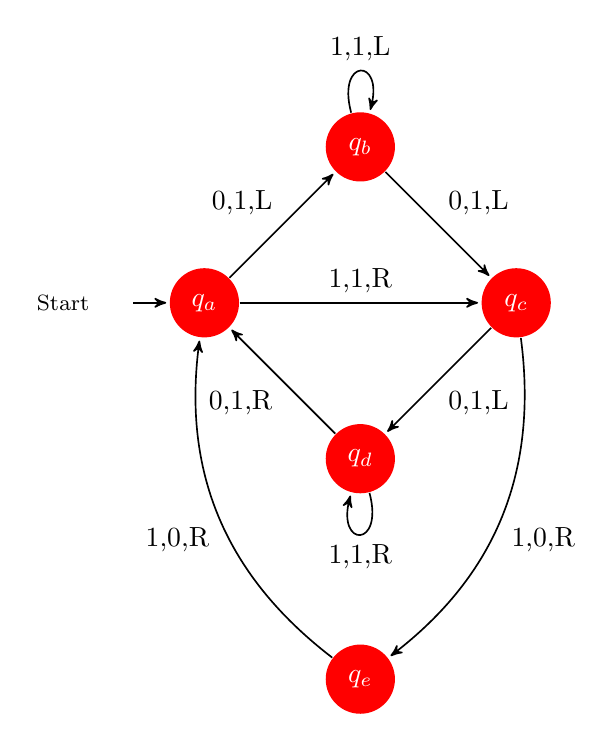
\begin{tikzpicture}[->,>=stealth',shorten >=1pt,auto,node distance=2.8cm,semithick]
			\tikzstyle{every state}=[fill=red,draw=none,text=white]
			\node[initial,state] (A) {$q_a$};
			\node[state] (B) [above right of=A] {$q_b$};
			\node[state] (D) [below right of=A] {$q_d$};
			\node[state] (C) [below right of=B] {$q_c$};
			\node[state] (E) [below of=D] {$q_e$};
			\path (A) edge node {0,1,L} (B)
			edge node {1,1,R} (C)
			(B) edge [loop above] node {1,1,L} (B)
			edge node {0,1,L} (C)
			(C) edge node {0,1,L} (D)
			edge [bend left] node {1,0,R} (E)
			(D) edge [loop below] node {1,1,R} (D)
			edge node {0,1,R} (A)
			(E) edge [bend left] node {1,0,R} (A);
			\node [left=1cm,text width=1cm,font=\footnotesize] at (A)
			{Start};
		\end{tikzpicture}
		\caption{Caption of the FSM}
	\end{figure}

	\begin{figure}[H]\centering
		\tikzstyle{pre} = [<-,shorten <=1pt,>=stealth',semithick]
		\tikzstyle{post} = [->,shorten >=1pt,>=stealth',semithick]
		\begin{tikzpicture}[->,>=stealth',shorten >=1pt,auto,node distance=3cm,semithick, bend angle=45]
			\tikzstyle{every state}=[fill=blue!20,draw=none,text=black]
			\node[state] (S0) {$S_0$}
				edge[loop left] node {$0/0$} (S0);
			\node[state] (S2) [above right of=S0] {$S_2$}
				edge[post, bend right] node[auto,swap] {$0/0$} (S0);
			\node[state] (S1) [below right of=S2] {$S_1$}
				edge[loop right] node {$1/0$} (S1)
				edge[pre, bend left] node[auto,swap] {$1/0$} (S0)
				edge[pre, bend left] node[auto,swap] {$1/1$} (S2)
				edge[post, bend right] node[auto,swap] {$0/0$} (S2);
		\end{tikzpicture}
		\caption{Caption of the FSM}
	\end{figure}

	\begin{figure}[H]\centering
		\tikzstyle{pre} = [<-,shorten <=1pt,>=stealth',semithick]
		\tikzstyle{post} = [->,shorten >=1pt,>=stealth',semithick]
		\begin{tikzpicture}[->,>=stealth',shorten >=1pt,auto,node distance=5cm,semithick, bend angle=45]
			\tikzstyle{every state}=[fill=none,draw=black,text=black]
			\node[state] (S0) {$estate$}
				edge[loop left] node {$in/out$} (S0);
			\node[state] (S1) [right of=S0] {$estate$}
				edge[loop right] node {$in/out$} (S1)
				edge[post, bend left] node[auto,swap] {$in/out$} (S0)
				edge[post, bend right] node[auto,swap] {$in/out$} (S0);

		\end{tikzpicture}
		\caption{Mealy Model}
	\end{figure}

\end{document}